%%%%%%%%%%%%%%%%%%%%%%%%%%%%%%%%%%%%%%%%%%%%%%
% Header
\documentclass[11pt]{report}
\usepackage[english]{babel}
\usepackage[utf8x]{inputenc}
\PassOptionsToPackage{hyphens}{url}\usepackage{hyperref}
\usepackage{graphicx}
\usepackage{fullpage}
\usepackage{nicefrac}
\usepackage[lastexercise]{exercise}
\usepackage[dvipsnames]{xcolor}
\usepackage{listings}

\setlength{\parindent}{0cm}

\renewcommand{\ExerciseHeader}{\large\textbf{\ExerciseName~\ExerciseHeaderNB} - \textbf{\ExerciseTitle}\medskip}

\renewcommand{\ExePartHeader}{\medskip\textbf{\ExePartName\ExePartHeaderNB\ExePartHeaderTitle\medskip}}

\begin{document}
%%%%%%%%%%%%%%%%%%%%%%%%%%%%%%%%%%%%%%%%%%%%%%
\title{Exercises -- Week 2: New Title}
\subsubsection*{EMAT10007 -- Introduction to Computer Programming}
\section*{\Large Solutions part 2:  Variables \& Types}


\begin{Exercise}[title=Variables] \label{Ex:Variables}
	\Question{Their respective values (10 and 5).}

	\Question{The value of x is overwritten and is now 4.}
	\Question{We get a Syntax error, because {\tt True} is a boolean keyword in python. }
		
	\Question{	{\tt x, y, z  = 5, 10, 15}}
\end{Exercise}

\begin{Exercise}[title=Numbers and Operators]

	\Question{{\tt A = 2}\\
	{\tt B = 3} (for example)}
	\Question{{\tt A+B}\\
	{\tt >>> 5}}
	\Question{{\tt A*(A+B)}\\
	{\tt >>> 10}}
	\Question{{\tt A*A+B}\\
	{\tt >>> 7}}
	\Question{{\tt A = 10}\\{\tt B = 3}\\  {\tt A/B} \\ {\tt >>>  3.3333333333333335}\\ {\tt A//B} \\ {\tt >>> 3}
	\Question{ {\tt A\%B}\\ {\tt >>> 1}}
	\Question{{\tt import math}\\ {\tt A = 5}\\ {\tt 2*A*math.pi}\\ {\tt >>> 31.41592653589793}}
\end{Exercise}

\begin{Exercise}[title=Booleans]
	\Question{{\tt A = 5}\\
	{\tt B = 4} (for example)}
    \Question{{\tt A < B}\\
    {\tt >>> True}\\
		    {\tt A > B}\\
		    {\tt >>> False}\\
		    {\tt A == B}\\
		    {\tt >>> False}\\
}
	\Question{The value of A is overwritten with the value of B (4 in this case).}
	\Question{The boolean value switches (from {\tt True} to {\tt False} or {\tt False} to {\tt True}.)}
	\Question{{\tt A = True} \\ {\tt B = False}\\
		\item Now try some logical (Boolean) operations such as:
		\begin{itemize}
		    \item {\tt A and B}\\
		    {\tt >>> False}
		    \item {\tt A or B}\\
		    {\tt >>> True}
		    \item {\tt A and not B}\\
		    {\tt >>> True}
		\end{itemize}}
	\Question{(*) {\tt bool(0)}\\
	{\tt >>> False}\\
    Any other number in the brackets evaluates as {\tt True}.}
\end{Exercise}

\subsection*{\Large Part 2:  Lists \& Strings}

\begin{Exercise}[title=Strings] \label{Ex:Strings}
	\Question{{\tt A = 'Hello'}\\
	 {\tt B = 'World'}}
	 \Question{{\tt type(A)}\\
	 {\tt >>> <class 'str'>}\\
	 {\tt type(B)}\\
	 {\tt >>> <class 'str'>}}
	\Question{{\tt A + B}\\
	{\tt >>> 'HelloWorld'}}
	\Question{We get a {\tt TypeError} as the multiplication operator is not defined for strings.}
	\Question{{\tt C = A + ' ' + B}}
	\Question{{\tt len(C)}\\
	{\tt >>> 11}}
	\Question{{\tt len()} works on sequences or collections, i.e. objects that are made up of a number of elements.}
	\Question{(*) 
	\begin{itemize}
	    \item {\tt "w" in C}\\
	    {\tt >>> False}
	    \item {\tt "hello" in C}\\
	    {\tt >>> False}
	    \item {\tt "Hello" in C}\\
	    {\tt >>> True}
	    \item {\tt "world" not in C}\\
	    {\tt >>> True}
	    \item {\tt A in C}\\
	    {\tt >>> True}
	\end{itemize}}
\end{Exercise}


\subsection*{\Large Exercises -- Week 2. More on Variables, Types and Conditionals}

\subsection*{\Large Part 1. Variables \& Types}

\setcounter{Exercise}{0}

\begin{Exercise}[title=Overwriting Variables] \label{Ex:Overwriting_Variables}
    \Question{ {\tt x = 5} \\
    {\tt x = x + 7}\\
    {\tt x = x - 3}\\
    {\tt x}
    {\tt >>> 9}
    }
    \Question{{\tt y = 2} \\
    {\tt y = y - 2}\\
    {\tt y += 2}\\
    {\tt y}\\
    {\tt >>> 2}
    
    {\tt +=} increments a variable by a set amount and {\tt -=} decrements a variable by a set amount.
    }
    \Question{{\tt x = 5} \\
    {\tt x += 7}\\
    {\tt x -= 3}\\}
    \Question{ {\tt y += y}\\?}
    \Question{We get a NameError as z has not been defined.
    }
    \Question{{\tt y *= 10}\\ {\tt y /= 5}\\}}
    \Question{(*) {\tt 8/2*(2+2)\\
    {\tt >>> 16.0}}
    }
\end{Exercise}

\begin{Exercise}[title=Naming Variables]
    \Question{\begin{itemize}
        \item {\tt cat name = "Whiskers"}
        \item {\tt cat-name = "Whiskers"}
        \item {\tt 1catname = "Whiskers"}
        \item {\tt \$catname = "Whiskers"}
        \item {\tt cat1 name = "Whiskers"}
        \item {\tt catname = "Whiskers"}
    \end{itemize}
    These all raise a {\tt SyntaxError} except for the last variable name as they contain characters which aren't allowed, spaces, or start with a number. 
    }
    \Question{{\tt catname} has not been overwritten, as Python is case-sensitive.}
    \Question{{\tt CatName = "Whiskers"}\\
    {\tt CatAge = 6}

    \textbf{Note:} {Kebab case uses hyphens which are not allowed in variable names in Python. }
    }
    \Question{ {\tt SPECIES = "cat"}}
    \Question{{\tt len = 10} does not produce an error}

\end{Exercise}

\begin{Exercise}[title=Number Types]
    \Question{ Use for example {\tt type(a)} to find the type of variable a.
    \begin{itemize}
        \item {\tt a} is of type int
        \item {\tt b} is of type float
        \item {\tt c} is of type complex
        \item {\tt d = 9j} is of type complex
        \item {\tt e = 0}  is of type int
        \item {\tt f = 2.0 + 0j} is of type complex
    \end{itemize}
    }
    \Question{{\tt y } is the only int.}
    \Question{We lose information when converting to "simpler" types, for instance from complex to float, float to int, complex to int, float to bool....}
    \Question{
    \begin{itemize}
        \item {\tt type(e)}\\
         {\tt >>> <class 'float'> }
        \item {\tt type(f)}\\
         {\tt >>> <class 'complex'> }
        \item {\tt type(g)}\\
         {\tt >>> <class 'float'> }
        \item {\tt type(h)}\\
         {\tt >>> <class 'float'> }
    \end{itemize}
    }
    \Question{(*) {\tt oct()}, {\tt hex()} and {\tt bin()} take ints as arguments and return a string containing the octal, hexadecimal and binary representation of the integer, respectively.}
\end{Exercise}

\begin{Exercise}[title=Boolean Operators]
    \Question{If you don't use capital letters for Boolean operators, you get a NameError. }
    \Question{
    \begin{itemize}
        \item {\tt A < B < C}\\
        {\tt >>> False}
        \item {\tt (A <= B) and (A > C)}\\
        {\tt >>> True}
        \item {\tt (2*A) == B}\\
        {\tt >>> True}
        \item {\tt A and B and C}\\
        {\tt >>> 0} (equivalent to False)
        \item {\tt (A != B) or C}\\
        {\tt >>> True}
        \item {\tt (A > 0) and (B > 0) or not (C == 0)}\\
        {\tt >>> True}
    \end{itemize}
    }
    \Question{(*) The {\tt xor} operator is equivalent to {\tt (a and not b) or (not a and b)}, and returns {\tt True} if one (and only one) of a, b are True.}
\end{Exercise}

\subsection*{\Large Part 2. Lists \& Strings}

\begin{Exercise}[title=Further Strings]
    \Question{\begin{itemize}
        \item {\tt str(4)}\\
        {\tt >>> '4'}
        \item {\tt 3.14159}\\
         {\tt >>> '3.14159'}
        \item {\tt 2+9j}\\
         {\tt >>> '(2+9j)'}
    \end{itemize}
    }
    \Question{Assigning a variable to just {\tt str()}creates an empty string.
    \Question{Use the str() function to convert ints to strings.
    }
    \Question{{\tt a[0]} accesses the first element.
    {\tt a[24]} accesses the last element, where 24 is {\tt len(a)-1}. We can also use {\tt a[-1]} to access the last element. 

    \Question{{\tt replace()} replaces elements within a string with other elements (i.e. characters).  Can you use it to change the {\tt a.replace('42','11')} will replace the value 42 in {\tt a} to 11 for instance.
    }
    \Question{(*) {\tt join()} connects strings using a character or string as a separator. Its usage takes some getting used to. If given a string as an argument, it will separate the string's characters. For instance: \\
   {\tt '/'.join('Eeny')}}\\
   {\tt >>> 'E/e/n/y'}\\
   To separate strings, one method is to make the strings part of a tuple: \\
   {\tt myRhymingTuple = ('Eeny','Meeny','Miny','Moe') }\\
     {\tt '/'.join(myRhymingTuple)}}\\
     {\tt >>> 'Eeny/Meeny/Miny/Moe'}
\end{Exercise}



\begin{Exercise}[title=Making a .py file]
    \Question{Self-explanatory. Refer to a lecturer or TA if you have any issues creating or saving files. 
\end{Exercise}

\subsection*{\Large Part 3. Control flow}

\begin{Exercise}[title=Conditionals]
    \Question{
    \vspace{1em}
    {\tt AgeOfWhiskers = 5}\\
    {\tt if AgeOfWhiskers <= 1.5:}\\
    \hspace*{2em} {\tt print("Whiskers is a kitten")}
    \vspace{1em}
    
 Nothing happens here, as AgeOfWhiskers doesn't satisfy the condition in the if statement. 
    }
    \Question{Add: \\
    {\tt else:}\\
     \hspace*{2em} {\tt print("Whiskers is an adult cat")}}\\
     The code now prints out:\\
     {\tt >>> "Whiskers is an adult cat"}
    \Question{Save as a file.}
    \vspace{-\baselineskip}
    \Question{Add between the if and else statements:\\
    \hspace*{2em} {\tt print("Whiskers is an old cat")}}
    \Question{Replace {\tt AgeOfWhiskers} with {\tt CatAge}}.
    \Question{(*) See the file "Circles.py" uppose we have three circles in the $xy$-plane. Circle $C_1$ is centred at $(0, 0)$ with radius of length 5. Circle $C_2$ is centred at $(2, 1)$ and has radius of length 2. Circle $C_3$ is centred at $(-5, 0)$ and has a radius of length 3. (See Figure \ref{fig:circles})
    
    Using conditional statements write a program which takes in the variables {\tt x} and {\tt y} and tests which circles the point $(x, y)$ is in. How can you make this as concise as possible? Are there any conditions you do not have to test?
    }
    \begin{figure}[!h]
        \centering
        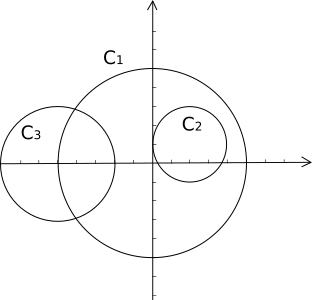
\includegraphics[height=5cm]{circles.png}
        \caption{Overlapping circles $C_1$, $C_2$ and $C_3$.}
        \label{fig:circles}
    \end{figure}}
\end{Exercise}




\end{document}